\documentclass[tikz, border=0]{standalone}
\usepackage{fontspec}
\usepackage{unicode-math}
\usepackage{pgfplots}
\pgfplotsset{compat=1.18}

\setmainfont{TeX Gyre Pagella}
\setmathfont{TeX Gyre Pagella Math}

\usetikzlibrary{calc,arrows.meta,patterns, decorations.markings}
\usetikzlibrary{luamath}

\definecolor{Red}{RGB}{ 159, 36, 48 }
\definecolor{Blue}{RGB}{ 103, 178, 255 }
\definecolor{LBlue}{RGB}{ 186, 220, 255 }
\definecolor{DBlue}{HTML}{132C53} 
\definecolor{gray}{HTML}{708090}
\definecolor{orange}{HTML}{ed9552}
\definecolor{orange2}{HTML}{e29d40}
\definecolor{PrintColor}{HTML}{000000}


\tikzset{
    axis/.style={ PrintColor, very thick, -{Stealth[length=1em,width=1em]} },
    plt/.style={ PrintColor, thick },
    sketch/.style={ gray, dashed , thick},
    flow/.style={
        plt,
        decoration={
            markings,
            mark=at position 0.17 with {\arrow{Stealth[length=0.5em,width=0.5em]}},
            mark=at position 0.5 with {\arrow{Stealth[length=0.5em,width=0.5em]}},
            mark=at position 0.83 with {\arrow{Stealth[length=0.5em,width=0.5em]}}
        },
        postaction={decorate}
    },
    stable manifold/.style={
        gray,
        thick,
        decoration={
            markings,
            mark=at position 0.17 with {\arrow{Stealth[length=1em,width=1em]}},
            mark=at position 0.33 with {\arrow{Stealth[length=1em,width=1em]}},
            mark=at position 0.67 with {\arrow{Stealth[reversed, length=1em,width=1em]}},
            mark=at position 0.83 with {\arrow{Stealth[reversed, length=1em,width=1em]}}
        },
        postaction={decorate}
    },
    unstable manifold/.style={
        gray,
        thick,
        decoration={
            markings,
            mark=at position 0.17 with {\arrow{Stealth[reversed, length=1em,width=1em]}},
            mark=at position 0.33 with {\arrow{Stealth[reversed, length=1em,width=1em]}},
            mark=at position 0.67 with {\arrow{Stealth[length=1em,width=1em]}},
            mark=at position 0.83 with {\arrow{Stealth[length=1em,width=1em]}}
        },
        postaction={decorate}
    },
}

\newcommand{\BeginMacros}{
        \pgfmathsetmacro{\Lx}{44}
        \pgfmathsetmacro{\Ly}{24}
        \pgfmathsetmacro{\xLim}{\Lx-2}
        \pgfmathsetmacro{\yLim}{\Ly-1}

        \useasboundingbox (-1,-1) rectangle (\Lx,\Ly);

        \coordinate (origin) at (0,0);
        \coordinate (ylim) at (0,\yLim);
        \coordinate (xlim) at (\xLim,0);
    }

\NewDocumentCommand{\SetAxis}{ O{$t$} O{$x$} }{
        \draw[font=\large,axis] (origin) -- (xlim)
            node[anchor=west] {#1};
        \draw[font=\large,axis] (origin) -- (ylim)
            node[anchor=north west, xshift=0.3em] {#2};
    }

\begin{document}

\begin{tikzpicture}[x=1em, y=1em]

    \BeginMacros

    \pgfmathsetseed{1195987779}

    \def\last{0}
    \foreach [count=\i] \t in {0.079825, 0.040892, 0.223986, 0.5, 0.155297} {
        \pgfmathsetmacro{\nextval}{\last + \t*\xLim}
        \pgfmathsetmacro{\h}{rnd*(\yLim-4)+3}

        \draw[plt] (\last, \h) -- (\nextval, \h) 
            node[color=PrintColor, midway, above] {$X_{\i}$};
        
        \draw[<->, gray, dashed, yshift=-1em] (\last, \h) -- (\nextval, \h)
            node[color=PrintColor, midway, below, yshift=0.1em] {$\Delta t_{\i}$};

        \draw[gray, dashed] (\last, 0) -- (\last, \h);
        \draw[gray, dashed] (\nextval, 0) -- (\nextval, \h);

        \xdef\last{\nextval}
    }

    \SetAxis[$t$][$X_t^{\text{r}}$]

\end{tikzpicture}

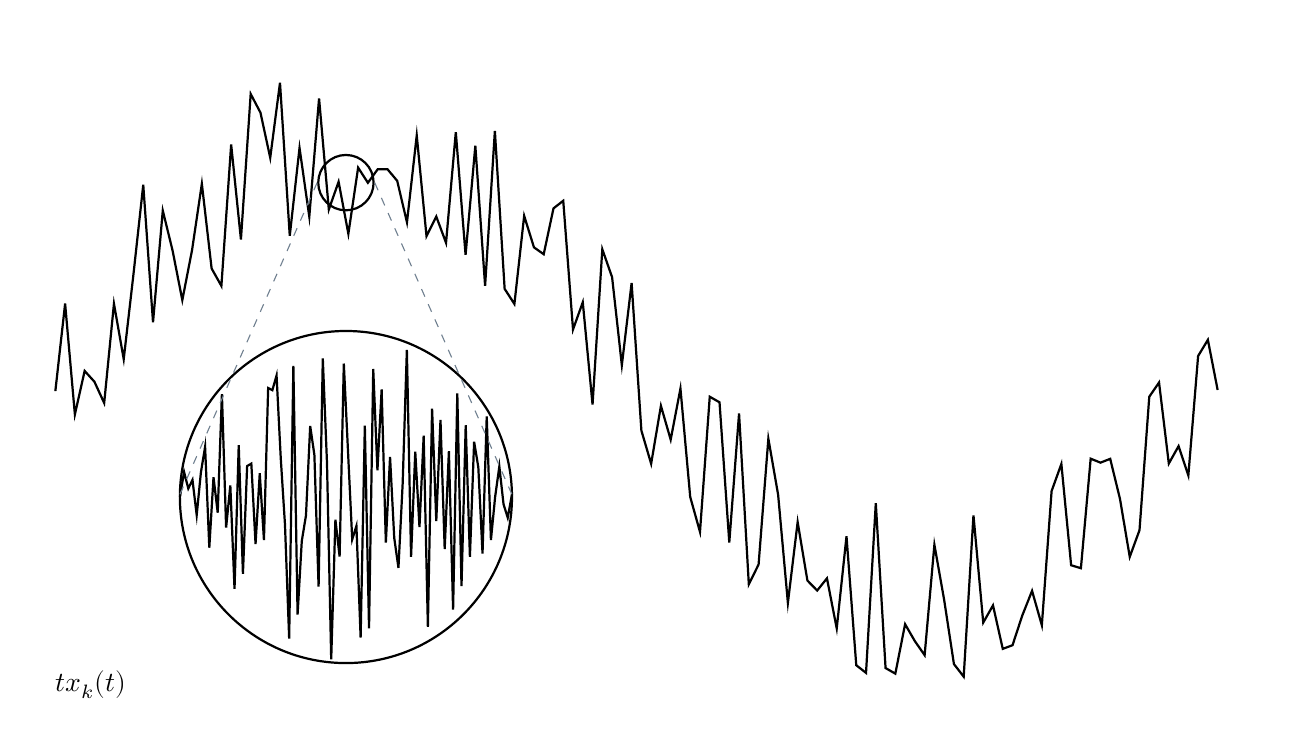
\begin{tikzpicture}[x=1em, y=1em]
    
    \BeginMacros

    \pgfmathsetseed{1195987779}

    \draw[plt] plot[domain=0:\xLim, samples=120]
        ({\x} , { 0.5*\yLim + 0.35*\yLim*( 0.4*rand + sin(360*\x/\xLim) ) });

    \node[circle, draw=PrintColor, thick, minimum size=2em] (look) at (0.25*\xLim,{0.8*\yLim}) {};

    \node[circle, draw=PrintColor, thick, minimum size=12em, anchor=south, yshift=1em] (zoom) at (0.25*\xLim,0) {};

    \begin{scope}[shift={(zoom.center)}]
        \draw[plt] plot[domain=-6:6, samples=80]
            ( {\x} , {sqrt(36-abs(\x)^2)*rand} );
    \end{scope}

    \draw[gray, dashed] (look.west) -- (zoom.west);
    \draw[gray, dashed] (look.east) -- (zoom.east);

    \SetAxis[$t$][$x_k(t)$]


\end{tikzpicture}

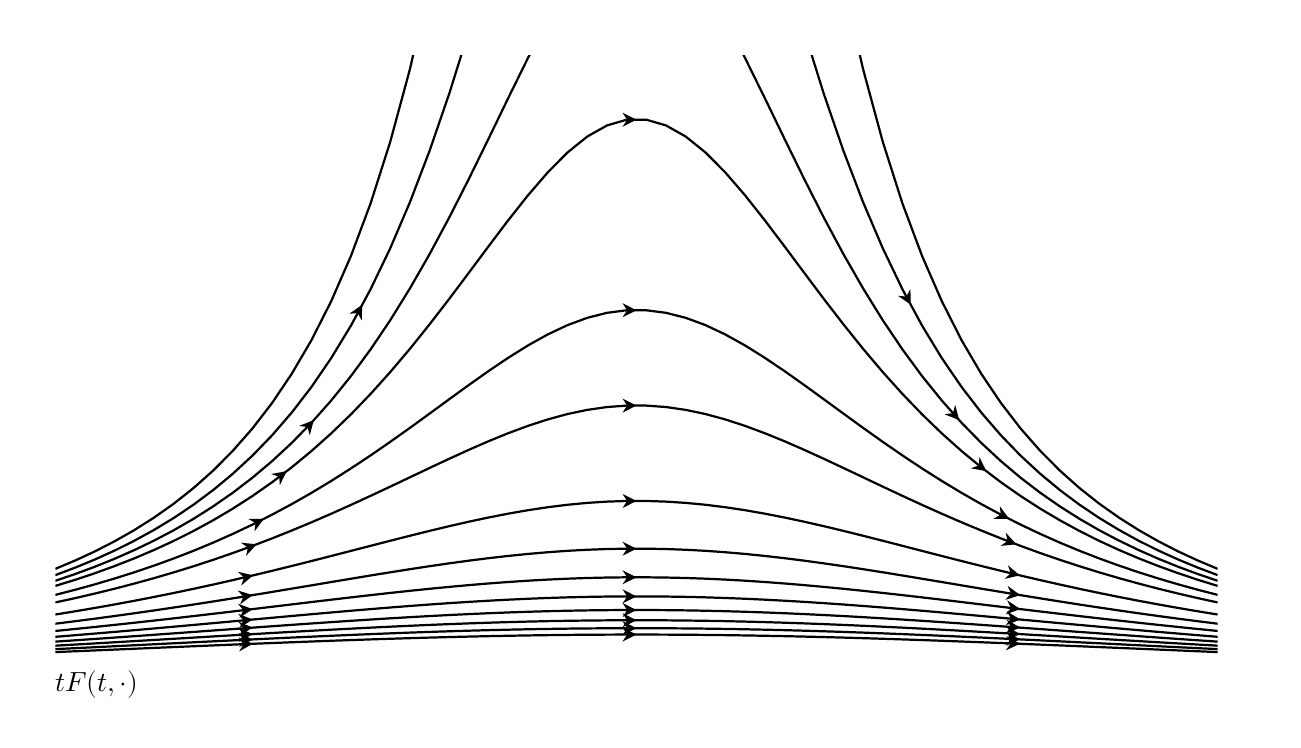
\begin{tikzpicture}[x=1em, y=1em]
    
    \BeginMacros

    \pgfmathsetseed{1195987779}

    \begin{scope}
    \clip (0,0) rectangle (\xLim,\yLim);
    \foreach \i in { 0.25,0.5,0.75,1,1.5,2,3,4,5,6,7,8,9,10 }{
        \draw[flow] plot[domain=0:\xLim, samples=60]
        ({\x} , { 0.9*\yLim/(0.01*(\x-0.5*\xLim)^2+\i) });
    }
    \end{scope}
    
    \SetAxis[$t$][$F(t,\cdot)$]
\end{tikzpicture}

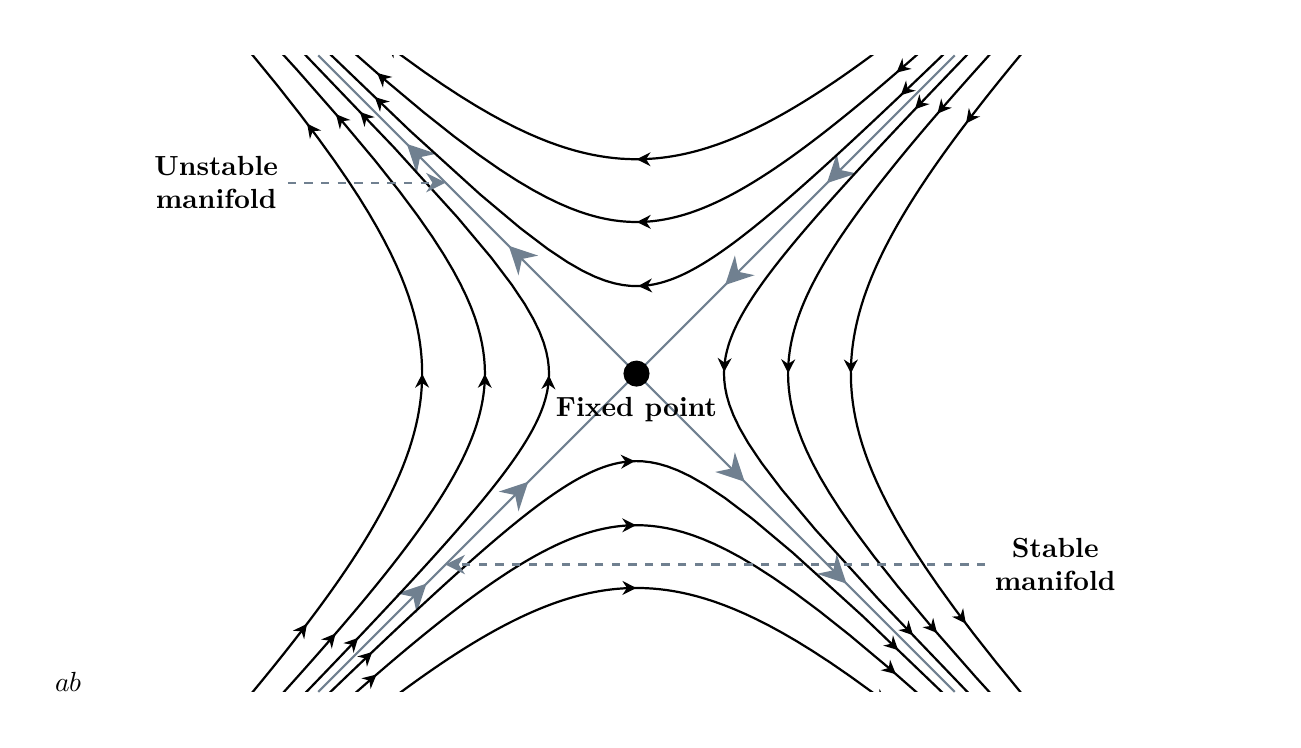
\begin{tikzpicture}[x=1em, y=1em]
    
    \BeginMacros

    \pgfmathsetmacro{\a}{0.5*\xLim}
    \pgfmathsetmacro{\b}{0.5*\yLim}

    \draw[stable manifold] (\a-\b,0) -- (\yLim+\a-\b,\yLim);
    \draw[unstable manifold] (-\yLim+\a+\b,\yLim) -- (\a+\b,0);

    \node[circle,fill=PrintColor,minimum size=0.1em] (fixed) at (\a,\b) {};
    \node[PrintColor, font=\bfseries, yshift=-0.8em] at (fixed.south) {Fixed point};

    \begin{scope}[shift={(fixed.center)}]
        \clip (-0.5*\xLim,-0.5*\yLim) rectangle (0.5*\xLim,0.5*\yLim);

        \foreach \C in { 5 , 15 , 30 }{
            \draw[flow] plot[domain=1/0.05:0.05*\C, samples=120]
                ({0.5*sqrt(2)*(\x-\C/\x)},{0.5*sqrt(2)*(\x+\C/\x)});
            \draw[flow] plot[domain=1/0.05:0.05*\C, samples=120]
                ({0.5*sqrt(2)*(-\x+\C/\x)},{0.5*sqrt(2)*(-\x-\C/\x)});
            
            \draw[flow] plot[domain=1/0.05:0.05*\C, samples=120]
                ({0.5*sqrt(2)*(\x+\C/\x)},{0.5*sqrt(2)*(\x-\C/\x)});
            \draw[flow] plot[domain=1/0.05:0.05*\C, samples=120]
                ({0.5*sqrt(2)*(-\x-\C/\x)},{0.5*sqrt(2)*(-\x+\C/\x)});
        }
    \end{scope}
    
    
    \node[PrintColor,font=\bfseries,anchor=east,align=center] (unstable) at (0.2*\xLim,0.8*\yLim) {Unstable\\ manifold};
    \node[PrintColor,font=\bfseries,anchor=west,align=center] (stable) at (0.8*\xLim,0.2*\yLim) {Stable\\ manifold};

    \draw[sketch, -{Stealth[length=0.7em,width=0.7em]}] (unstable.east) -- (-0.8*\yLim+\a+\b,0.8*\yLim);
    \draw[sketch, -{Stealth[length=0.7em,width=0.7em]}] (stable.west) -- (0.2*\yLim+\a-\b,0.2*\yLim);


    \SetAxis[$a$][$b$]
\end{tikzpicture}

\end{document}